\section{\textbf{System Modeling}}
\label{sec:systemModel}

A sequential and iterative design process was adopted to refine simulation model and mechanical design as shown in Figure \ref{fig:systemOverview}. The 1-DOF template \cite{Full1999} called \textbf{knee extensor model} was used to investigate the torque and angular speed requirement of the leg, as depicted in Figure \ref{fig:systemOverview}(a). It assumes all masses are lumped at the base; thigh and shank link are of same length and have no mass or inertia; foot is located directly below the hip, which means no horizontal off-set for foot hold. Jumping motion was simulated using this knee extensor model under various motors' maximal speed and maximal torque. These simulations in turn exposed the speed and torque requirements in order to achieve the desired motion, which provides guidance for choosing appropriate motor and gear ratio.

A more detailed leg model with motors' rotary inertia and horizontal foot off-set was introduced as shown in Figure \ref{fig:systemOverview} (b). The detailed leg model was used to further narrow the choice of gear ratio by minimizing ground impact force while maintaining balance between torque and speed requirements. Optimized parameters were tested on the hardware platform shown in Figure \ref{fig:systemOverview} (c) to validate the design.

\begin{figure}
	\centering
	\resizebox{1.0\linewidth}{!}{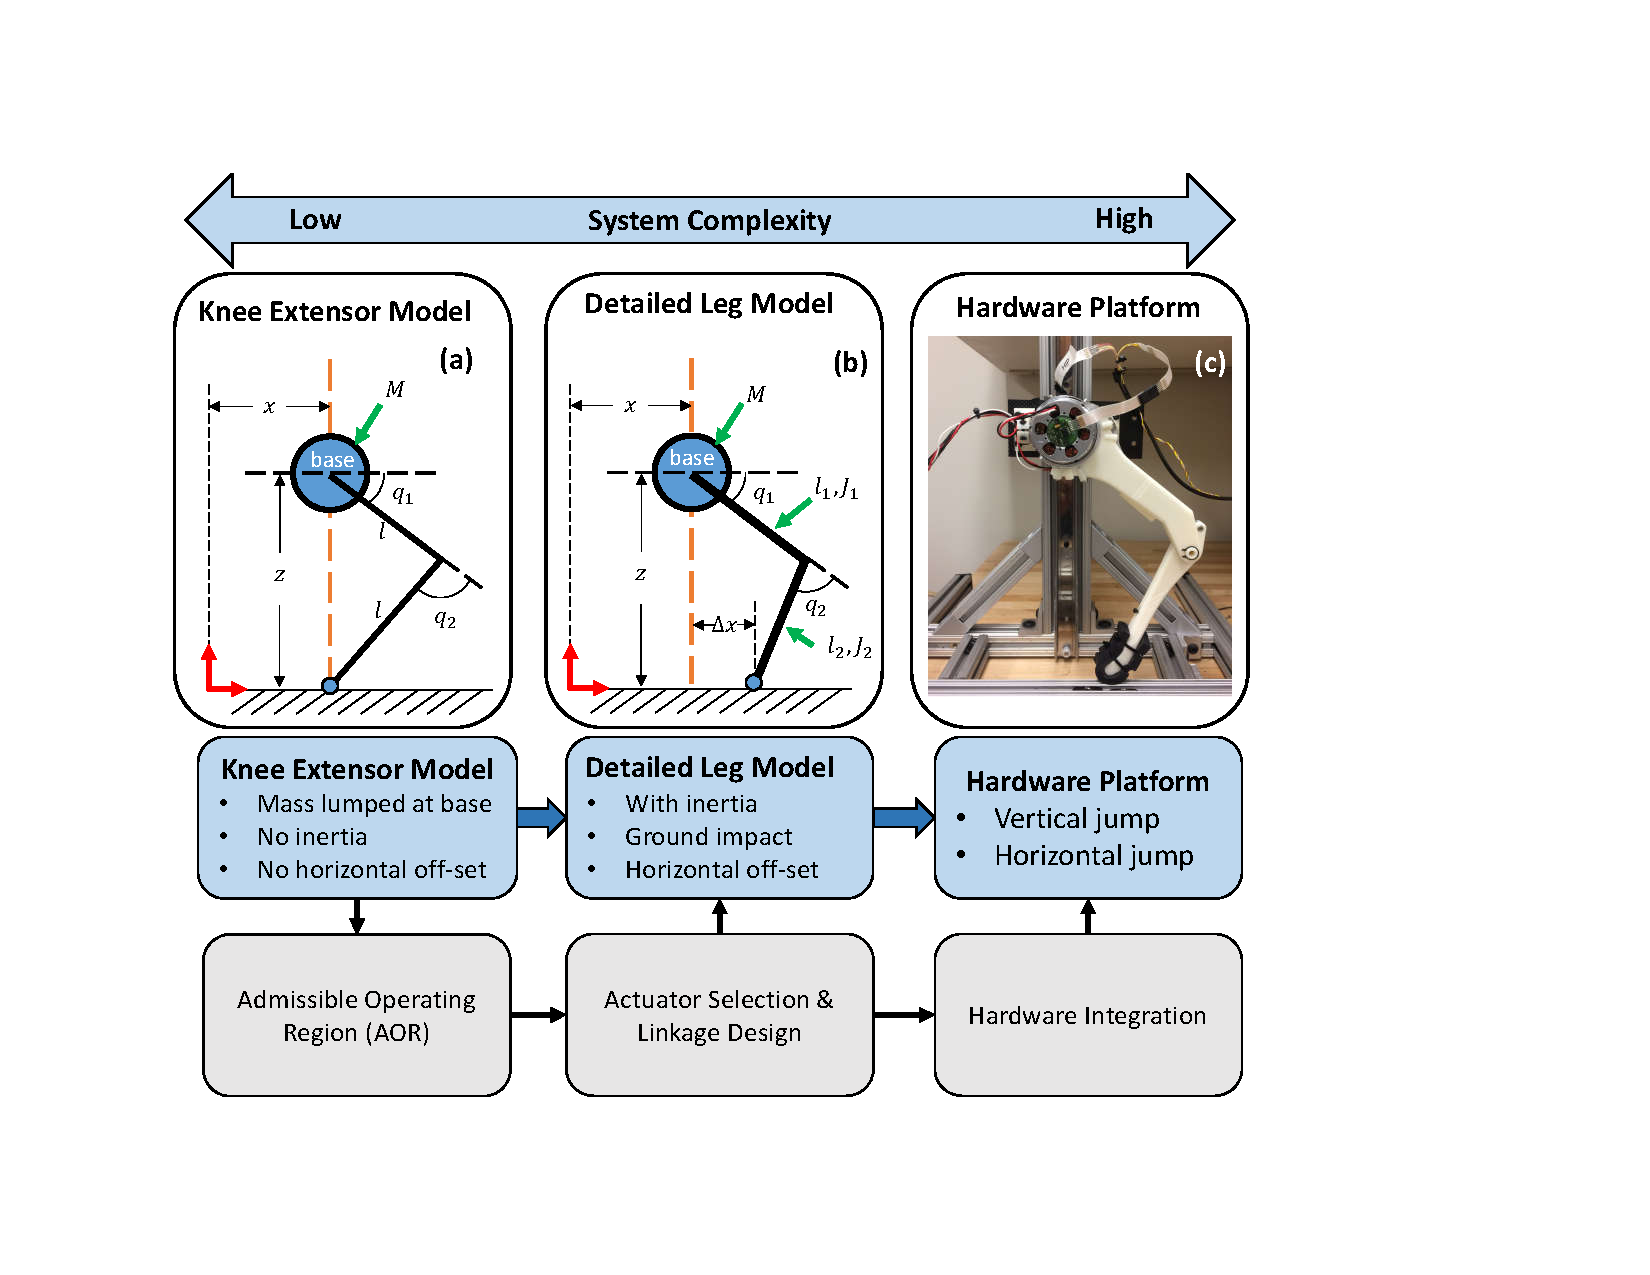
\includegraphics{system_overview.pdf}}
	\caption{Sequential design process for determining design parameters. (a) knee extensor model for motor selection (b) detailed leg model for linkage design and gear ratio choice (c) hardware platform for experiments}
	\label{fig:systemOverview}
\end{figure}

\subsection{Knee Extensor Model}
\label{sec:kneeExtensorModel}

The knee extensor model was used to estimate the torque and speed requirements to achieve desirable jumping motions, which provides us with an initial guidance for choosing motor and gearbox. Figure \ref{fig:systemOverview} (a) shows the schematics of the knee extensor model. The model assumes that all masses are lumped at the base to be $M$, which is mounted on a vertical linear rail. Thigh and shank links have an identical length of $l$, while its foot and base are vertically aligned. Hence only the knee joint needs to be actuated to perform vertical jump while the hip joint is not actuated. The vertical height of the base $z$ and joint angles $q_1, q_2$ are shown in Figure \ref{fig:systemOverview}.

The dynamics of this model was formalized as a single point mass accelerated due to ground reaction force (GRF). Ground reaction force was chosen as the control input because it is the only external force in the knee extensor model that could increase the mechanical energy of the system. The equation of motion (EOM) of the system is: $\ddz = \frac{F_z}{M}-g$, where $z$ is the vertical displacement of the base, $F_z$ is the vertical component of GRF, $M$ is the lumped mass at the base and $g$ is the gravitational acceleration. 

\subsection{GRF Parameterized as \Bezier\ Polynomial}
\label{sec:BezierPoly}
	
A $5^{th}$ order \Bezier\ polynomial was used to parameterize the GRF profile. The reasons for using \Bezier\ Polynomial to parametrize the ground reaction force is two fold. Firstly, the first and last coefficient of a \Bezier\ polynomial corresponds to the initial and final value of the GRF, which makes it more convenient to anchor GRF to desired values at the initial and final instance; secondly, integration of \Bezier\ Polynomial is a linear operation, which is computationally inexpensive.

The coefficients of \Bezier\ polynomial are assumed to be $[Mg, \alpha_1, \alpha_2, \alpha_3, \alpha_4, 0]$. The first coefficient was set to be the weight of the leg because it is assumed that the leg starts from static equilibrium state, and last coefficient was set as $0$ to ensure a smooth and physically feasible motion at the take-off moment.  

Since a \Bezier\ polynomial is the linear combination of a Bernstein polynomial basis\cite{dicsibuyuk2007generalization} defined as,

\begin{equation}\label{eq:bezier}
C_N(s) = \sum_{i=0}^{N}\alpha_i B_{i,N}(s)
\end{equation}

where $\alpha_i$ is the coefficient for the $i^{th}$ Bernstein polynomial $B_{i,N}$, analytical solution for velocity and position could be obtained using the property of the Bernstein polynomial\cite{Doha2011}:

\begin{equation} \label{eq:bernstein_diff}
\frac{d}{ds}B_{i,N}(s)=\frac{N}{T}(B_{i-1,N-1}(s)-B_{i,N-1}(s))
\end{equation}
where $s$ is a point between general time interval $[0, T]$.

Given the initial velocity $\dz_0$, the velocity trajectory in stance phase is a $6^{th}$ order \Bezier\ polynomial with coefficients $\gamma_{(0-6)}$. The linear relationship between force and velocity \Bezier\ coefficient is:

\begin{equation}\label{eq:bernstein_integration}
\frac{6}{T_{st}}\left[
\begin{smallmatrix}
-1 & 1 & 0 & 0 & 0 & 0 & 0 \\
0 &-1 & 1 & 0 & 0 & 0 & 0 \\
0 & 0 &-1 & 1 & 0 & 0 & 0 \\
0 & 0 & 0 &-1 & 1 & 0 & 0 \\
0 & 0 & 0 & 0 &-1 & 1 & 0 \\
0 & 0 & 0 & 0 & 0 &-1 & 1 \\
1 & 0 & 0 & 0 & 0 & 0 & 0 \\
\end{smallmatrix}
\right]
\left[
\begin{matrix}
\gamma_0\\\gamma_1\\\gamma_2\\\gamma_3\\\gamma_4\\\gamma_5\\\gamma_6\\
\end{matrix}
\right]
=
\left[
\begin{matrix}
\left[
\begin{matrix}
0\\\alpha_1\\\alpha_2\\\alpha_3\\\alpha_4\\0\\
\end{matrix}
\right]\frac{1}{M}-g\\
\dz_0\\
\end{matrix}
\right]
\end{equation}
where $T_{st}$ is the stance duration for jumping up.

Similarly, the position trajectory in stance phase could also be retrieved by applying the linear operation shown in Equation \ref{eq:bernstein_integration} given initial position $z_0$. At each instance  $t\in[0,T_{st} ]$, the joint angle $q=[q_1,q_2]$ defined in Figure \ref{fig:systemOverview}(a) was solved by inverse kinematics. Since the thigh and shank links are assumed to be massless, joint torque $\tau=[\tau_1,\tau_2]$ could be reconstructed using $\tau=J(q)^T F$, where $\tau_1$ and $\tau_2$ are joint torques for hip and knee joints, $F$ is the ground reaction force, and $J(q)\in R^{2\times 2} $ is the manipulator Jacobian of the foot relative to the hip.

The jumping performance was evaluated by the maximal reachable height $h_{max}$, $h_{max} := h_{to}+\frac{v_{to}^2}{2g}$ where $h_{to}$ and $v_{to}$ are the base height and speed at the moment of take-off.


\subsection{Nonlinear Optimization for Ground Reaction Force}
\label{sec:nonlOptGRF}

\begin{figure}
	\centering
	\resizebox{1.0\linewidth}{!}{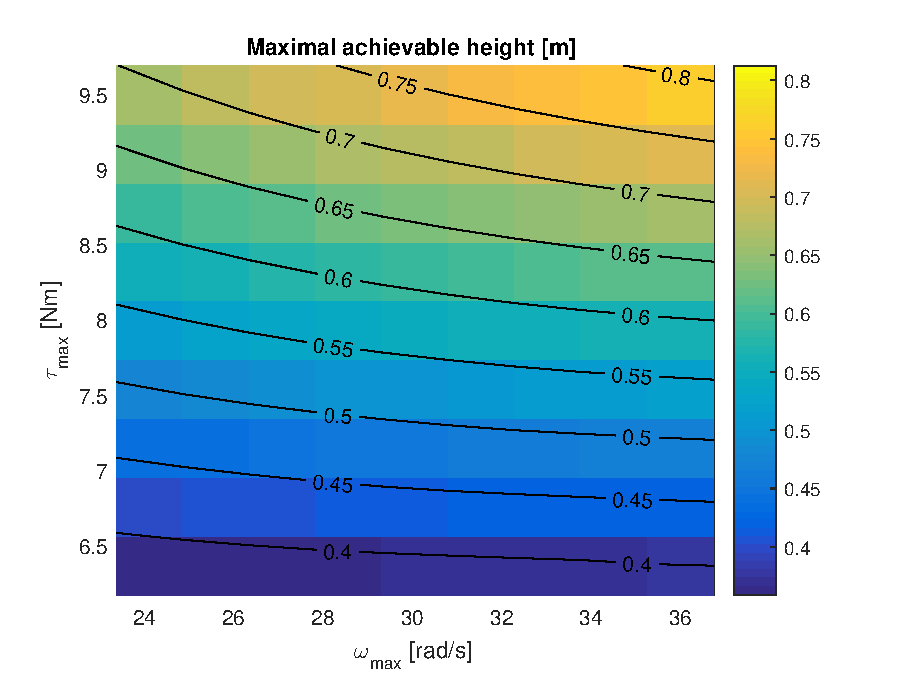
\includegraphics{hmax_pcolor.eps}}
	\caption{Maximal achievable height for specific torque and speed limit. The x-axis corresponds to maximal angular velocity of the actuator, the y-axis corresponds to maximal torque of the actuator, and the depth represents the maximal achievable height of a jump}
	\label{fig:hmax_pcolor}
\end{figure}




